\chapter{Probability Distributions}\label{c2}
\section{Problems}\label{c2p}
\begin{enumerate}
\item The Bernoulli distribution is defined as $\mathrm{Bern}(x|\mu) = \mu^x(1 - \mu)^x$. The 
random variable can take only two values, $0$ and $1$. Clearly, $p(X=0|\mu) = 1 - \mu$ and 
$p(X=1|\mu) = \mu$ so that
\[
\sum_x p(x|\mu) = 1.
\]
The expectation value of $X$ is
\[
\ev(X) = \sum_x xp(x|\mu) = 0\cdot(1 - \mu) + 1\cdot\mu = \mu.
\]
The variance of $X$ is
\[
\var(X) = \sum_x \ev(x - \mu)^2 = (0 - \mu)^2(1 - \mu) + (1 - \mu)^2\mu = \mu(1 - \mu).
\]

\item Given that
\[
p(x|\mu) = \left(\frac{1-\mu}{2}\right)^{(1-x)/2}\left(\frac{1+\mu}{2}\right)^{(1+x)/2},
\]
where $x \in {-1, 1}$ and $\mu \in [0, 1]$. Then $p(X=-1|\mu) = (1 - \mu)/2$ and $p(X=1|\mu)
= (1 + \mu)/2$ so that 
\[
\sum_x p(x|\mu) = 1.
\]
The expectation value of $X$ is
\[
\ev(X) = \sum_x xp(x|\mu) = -1\cdot\frac{1 - \mu}{2} + 1\cdot\frac{1 + \mu}{2} = \mu.
\]
We also find
\[
\ev(X^2) = \frac{1 - \mu}{2} + \frac{1 + \mu}{2} = 1
\]
so that $\var(X) = 1 - \mu^2$. We verify the variance using the other form,
\[
\var(X) = (-1 - \mu)^2\frac{1 - \mu}{2} + (1 - \mu)^2\frac{1 + \mu}{2} = 1 - \mu^2.
\]

\item We can show that the binomial distribution is normalized by evaluating the sum,
\[
\sum_{m=0}^N\binom{N}{m}\mu^m(1 - \mu)^{N-m} = (\mu + 1 - \mu)^N = 1.
\]
We used the binomial theorem to get the first equality.

\item Consider the expression,
\[
\sum_{k=0}^N \binom{N}{k}\mu^k(1 - \mu)^{N-k} = 0.
\]
Differentiate it with respect to $\mu$. Recall that $\mu \in [0, 1]$ so that the differentiation 
is well defined.
\[
\sum_{k=0}^N\binom{N}{k}k\mu^{k-1}(1 - \mu)^{N-k} - \sum_{k=0}^N\binom{N}{k}(N-k)\mu^k(1 - \mu)^{N-k-1} = 0.
\]
Multiply throughout by $\mu$ to get
\[
\sum_{k=0}^N\binom{N}{k}\mu^k(1 - \mu)^{N-k} = \mu N\sum_{k=0}^{N-1}\binom{N-1}{k}\mu^k(1 - \mu)^{N-k-1}.
\]
The left hand side is $\bar{X}$ while the right hand side is $\mu N$.

\item Consider the product
\[
\Gamma(a)\Gamma(b) = \int_0^\infty e^{-x}x^{a-1}dx\int_0^\infty e^{-y}y^{b-1}dy = \iint_{Q_1}e^{-x-y} x^{a-1}y^{b-1}dxdy,
\]
where $Q_1$ is the first quadrant. To evaluate this integral, introduce the variables $x = zt$
and $y = z(1 - t)$ or $z = x + y$ and $t = x/(x + y)$. The variable $z$ ranges from $0$ to 
$\infty$ while $t$ goes from $0$ to $1$. The jacobian of the transformation is
\[
\frac{\partial(x, y)}{\partial(z, t)} = \begin{vmatrix} x_z & x_t \\ y_z & y_t \end{vmatrix}
= \begin{vmatrix} t & z \\ 1 - t & -z \end{vmatrix} = -z.
\]
Therefore, 
\[
\Gamma(a)\Gamma(b) = \int_0^\infty\int_0^1 e^{z} z^{a-1}t^{a-1}z^{b-1}(-t)^{b-1}\abs*{\frac{\partial(x, y}{\partial(z, t)}}dzdt.
\]
The $z$ and the $t$ integrals factor out, so that
\[
\Gamma(a)\Gamma(b) = \int_0^\infty e^z z^{a+b-1}dz\int_0^1 t^{a-1}(1 - t)^{b- 1}dt = \Gamma(a+b)B(a, b).
\]

\item The mean of beta distribution is
\begin{eqnarray*}
\ev(X) &=& \frac{\Gamma(a+b)}{\Gamma(a)\Gamma(b)}\int_0^1 x B(x|a, b)dx \\
 &=& \frac{\Gamma(a+b)}{\Gamma(a)\Gamma(b)}\int_0^1x^a(1 - x)^{b-1}dx \\
 &=& \frac{\Gamma(a+b)}{\Gamma(a)\Gamma(b)}\frac{\Gamma(a+1)\Gamma(b)}{\Gamma(a+b+1)} \\
 &=& \frac{a}{a+b}.
\end{eqnarray*}
Likewise,
\begin{eqnarray*}
\ev(X^2) &=& \frac{\Gamma(a+b)}{\Gamma(a)\Gamma(b)}\int_0^1 x^2 B(x|a, b)dx \\
 &=& \frac{\Gamma(a+b)}{\Gamma(a)\Gamma(b)}\int_0^1x^{a+2}(1 - x)^{b-1}dx \\
 &=& \frac{\Gamma(a+b)}{\Gamma(a)\Gamma(b)}\frac{\Gamma(a+2)\Gamma(b)}{\Gamma(a+b+2)} \\
 &=& \frac{a(a+1)}{(a+b)(a+b+1)}.
\end{eqnarray*}
Therefore,
\[
\var{X} = \frac{a(a+1)}{(a+b)(a+b+1)} - \frac{a^2}{(a+b)^2} = \frac{ab}{(a+b)^2(a+b+1)}.
\]

The mode of the distribution is the maximum of $\mathrm{Beta}(X|a, b)$. Its derivative
with respect to $x$ is
\[
\frac{\Gamma(a+b)}{\Gamma(a)\Gamma(b)}\left((a-1)x^{a-2}(1-x)^{b-1} - (b-1)x^{a-1}(1-x)^{b-2}\right)
\]
The extremum is found by setting it equal to zero, which gives
\[
(a-1)(1 - x) = (b - 1)x
\]
or
\[
x = \frac{a-1}{a+b-2}.
\]

We can use the following R code to generate plots of beta distributions for various
values of $a$ and $b$.
\begin{lstlisting}[language=R, frame=single]
x <- seq(from = 0, to = 1, by = 0.01)
b.1 <- dbeta(x, 0.1, 0.1)
b.2 <- dbeta(x, 1, 1)
b.3 <- dbeta(x, 2, 3)
b.4 <- dbeta(x, 8, 4)
plot(x, 
     b.1, 
     type = "l", 
     xlab = "x", 
     ylab = "B(a, b)", 
     main = "Beta distributions")
lines(x, b.2, col = 2, lty = 2)
lines(x, b.3, col = 3, lty = 3)
lines(x, b.4, col = 4, lty = 4)
legend(locator(1), 
       legend = c("(0.1,0.1)","(1,1)","(2,3)","(8,4)"), 
       col = c(1,2,3,4), 
       lty = c(1,2,3,4), 
       cex = 0.7, 
       bty = "n")
\end{lstlisting}

\begin{figure}
\begin{center}
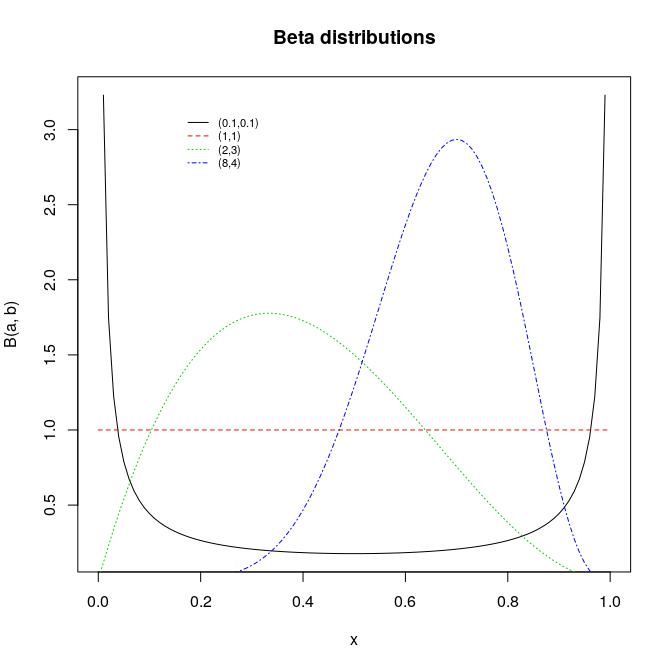
\includegraphics[scale=0.4]{c2f1}
\end{center}
\end{figure}

\end{enumerate}

